% Generated by render.py; edit preamble.tex, citations.json and route.tikz
\documentclass[border=12pt]{standalone}
\def\pgfsysdriver{pgfsys-dvisvgm.def}
\usepackage[dvisvgm]{xcolor}
\usepackage{xeCJK}
\setCJKmainfont{HaranoAjiGothic-Regular.otf}[BoldFont=HaranoAjiGothic-Bold.otf]
\setCJKsansfont{HaranoAjiGothic-Regular.otf}[BoldFont=HaranoAjiGothic-Bold.otf]
\usepackage{amsmath,amssymb,tikz,lmodern}
\usetikzlibrary{arrows.meta,positioning,calc,fit,backgrounds}
\renewcommand{\familydefault}{\sfdefault}
\definecolor{ink}{HTML}{25322F}
\definecolor{green}{HTML}{246657}
\definecolor{tint}{HTML}{EEF4F0}
\definecolor{soft}{HTML}{C6D2CC}
\definecolor{muted}{HTML}{52615B}
\newif\ifJapanese
\newcommand{\Tx}[2]{\ifJapanese #1\else #2\fi}
\newcommand{\Eff}{\overline{\operatorname{Eff}}}
\newcommand{\heading}[3]{{\color{green}\bfseries #1\quad\Tx{#2}{#3}}\\[5pt]}
% A white rectangle makes the complete citation label clickable, including spaces.
\newcommand{\refurl}[2]{\special{dvisvgm:raw <a xlink:href="#1" target="_blank" rel="noopener noreferrer">}{\setlength{\fboxsep}{0pt}\colorbox{white}{\color{green}\underline{\strut #2}}}\special{dvisvgm:raw </a>}}
\tikzset{
 card/.style={draw=soft,fill=white,rounded corners=2pt,align=left,text=ink,font=\fontsize{10.5}{14}\selectfont,inner xsep=12pt,inner ysep=10pt,text width=14.4cm},
 half/.style={card,text width=6.45cm,minimum height=2.05cm},
 result/.style={card,draw=green,fill=tint,line width=.9pt},
 reason/.style={align=left,text=muted,font=\fontsize{9}{12}\selectfont,inner sep=0pt,text width=12.6cm},
 branchreason/.style={reason,text width=5.95cm},
 edge/.style={-{Stealth[length=2.4mm]},draw=green,line width=1pt},
 wire/.style={draw=green,line width=1pt},
}
% Keep the arrow in a dedicated left gutter; explanations never cover it.
\def\flow#1#2#3;{
 \coordinate (#2-from) at ($(#1.south)+(-6.9,0)$);
 \coordinate (#2-to) at ($(#2.north)+(-6.9,0)$);
 \draw[edge] (#2-from)--(#2-to);
 \node[reason,anchor=west] (#2-reason) at ($(#2-from)!.5!(#2-to)+(.55,0)$) {#3};
}

% Style adapted from the repository's Schnell diagrams; MIT attribution retained.

% Generated from citations.json; do not edit.
\newcommand{\Cite}[1]{\csname cite-#1\endcsname}
\expandafter\def\csname cite-pointwise-main\endcsname{\shortstack[l]{\refurl{https://github.com/openai/math/blob/1581d4cbdd69a0faf34b2089614fe2a814316a6a/preprints/A-pointwise-2-converse-for-elliptic-curves-with-rational-two-torsion-October-7-2026/paper.pdf}{[OpenAI26P, Theorem 1.1, p. 2]}}}
\expandafter\def\csname cite-hilbert-main\endcsname{\shortstack[l]{\refurl{https://github.com/openai/math/blob/1581d4cbdd69a0faf34b2089614fe2a814316a6a/preprints/Hilberts-tenth-problem-over-the-rational-numbers-October-6-2026/main.pdf}{[OpenAI26H, Theorem 1.1, p. 3]}}}
\expandafter\def\csname cite-hilbert-transfer\endcsname{\shortstack[l]{\refurl{https://github.com/openai/math/blob/1581d4cbdd69a0faf34b2089614fe2a814316a6a/preprints/Hilberts-tenth-problem-over-the-rational-numbers-October-6-2026/main.pdf}{[OpenAI26H, Lemma 3.4, pp. 23–24]}}}
\expandafter\def\csname cite-hilbert-poles\endcsname{\shortstack[l]{\refurl{https://github.com/openai/math/blob/1581d4cbdd69a0faf34b2089614fe2a814316a6a/preprints/Hilberts-tenth-problem-over-the-rational-numbers-October-6-2026/main.pdf}{[OpenAI26H, Proposition 2.8, p. 12]}}}
\expandafter\def\csname cite-hilbert-local\endcsname{\shortstack[l]{\refurl{https://github.com/openai/math/blob/1581d4cbdd69a0faf34b2089614fe2a814316a6a/preprints/Hilberts-tenth-problem-over-the-rational-numbers-October-6-2026/main.pdf}{[OpenAI26H, Lemma 2.10; Proposition 2.11, pp. 14–15]}}}
\expandafter\def\csname cite-hilbert-height\endcsname{\shortstack[l]{\refurl{https://github.com/openai/math/blob/1581d4cbdd69a0faf34b2089614fe2a814316a6a/preprints/Hilberts-tenth-problem-over-the-rational-numbers-October-6-2026/main.pdf}{[OpenAI26H, Theorem 2.4, p. 9]}}}
\expandafter\def\csname cite-hilbert-tests\endcsname{\shortstack[l]{\refurl{https://github.com/openai/math/blob/1581d4cbdd69a0faf34b2089614fe2a814316a6a/preprints/Hilberts-tenth-problem-over-the-rational-numbers-October-6-2026/main.pdf}{[OpenAI26H, §2.4; Proposition 2.12, pp. 12–17]}}}
\expandafter\def\csname cite-hilbert-degree\endcsname{\shortstack[l]{\refurl{https://github.com/openai/math/blob/1581d4cbdd69a0faf34b2089614fe2a814316a6a/preprints/Hilberts-tenth-problem-over-the-rational-numbers-October-6-2026/main.pdf}{[OpenAI26H, Corollary 7.1, pp. 56–57]}}}
\expandafter\def\csname cite-hilbert-completion\endcsname{\shortstack[l]{\refurl{https://github.com/openai/math/blob/1581d4cbdd69a0faf34b2089614fe2a814316a6a/preprints/Hilberts-tenth-problem-over-the-rational-numbers-October-6-2026/main.pdf}{[OpenAI26H, §3.4, pp. 24–26]}}}
\expandafter\def\csname cite-official\endcsname{\shortstack[l]{\refurl{https://github.com/openai/math/blob/1581d4cbdd69a0faf34b2089614fe2a814316a6a/overview.pdf}{OpenAI Research Catalog · Catalogue 004 · p. 2}}}

\Japanesetrue
\begin{document}
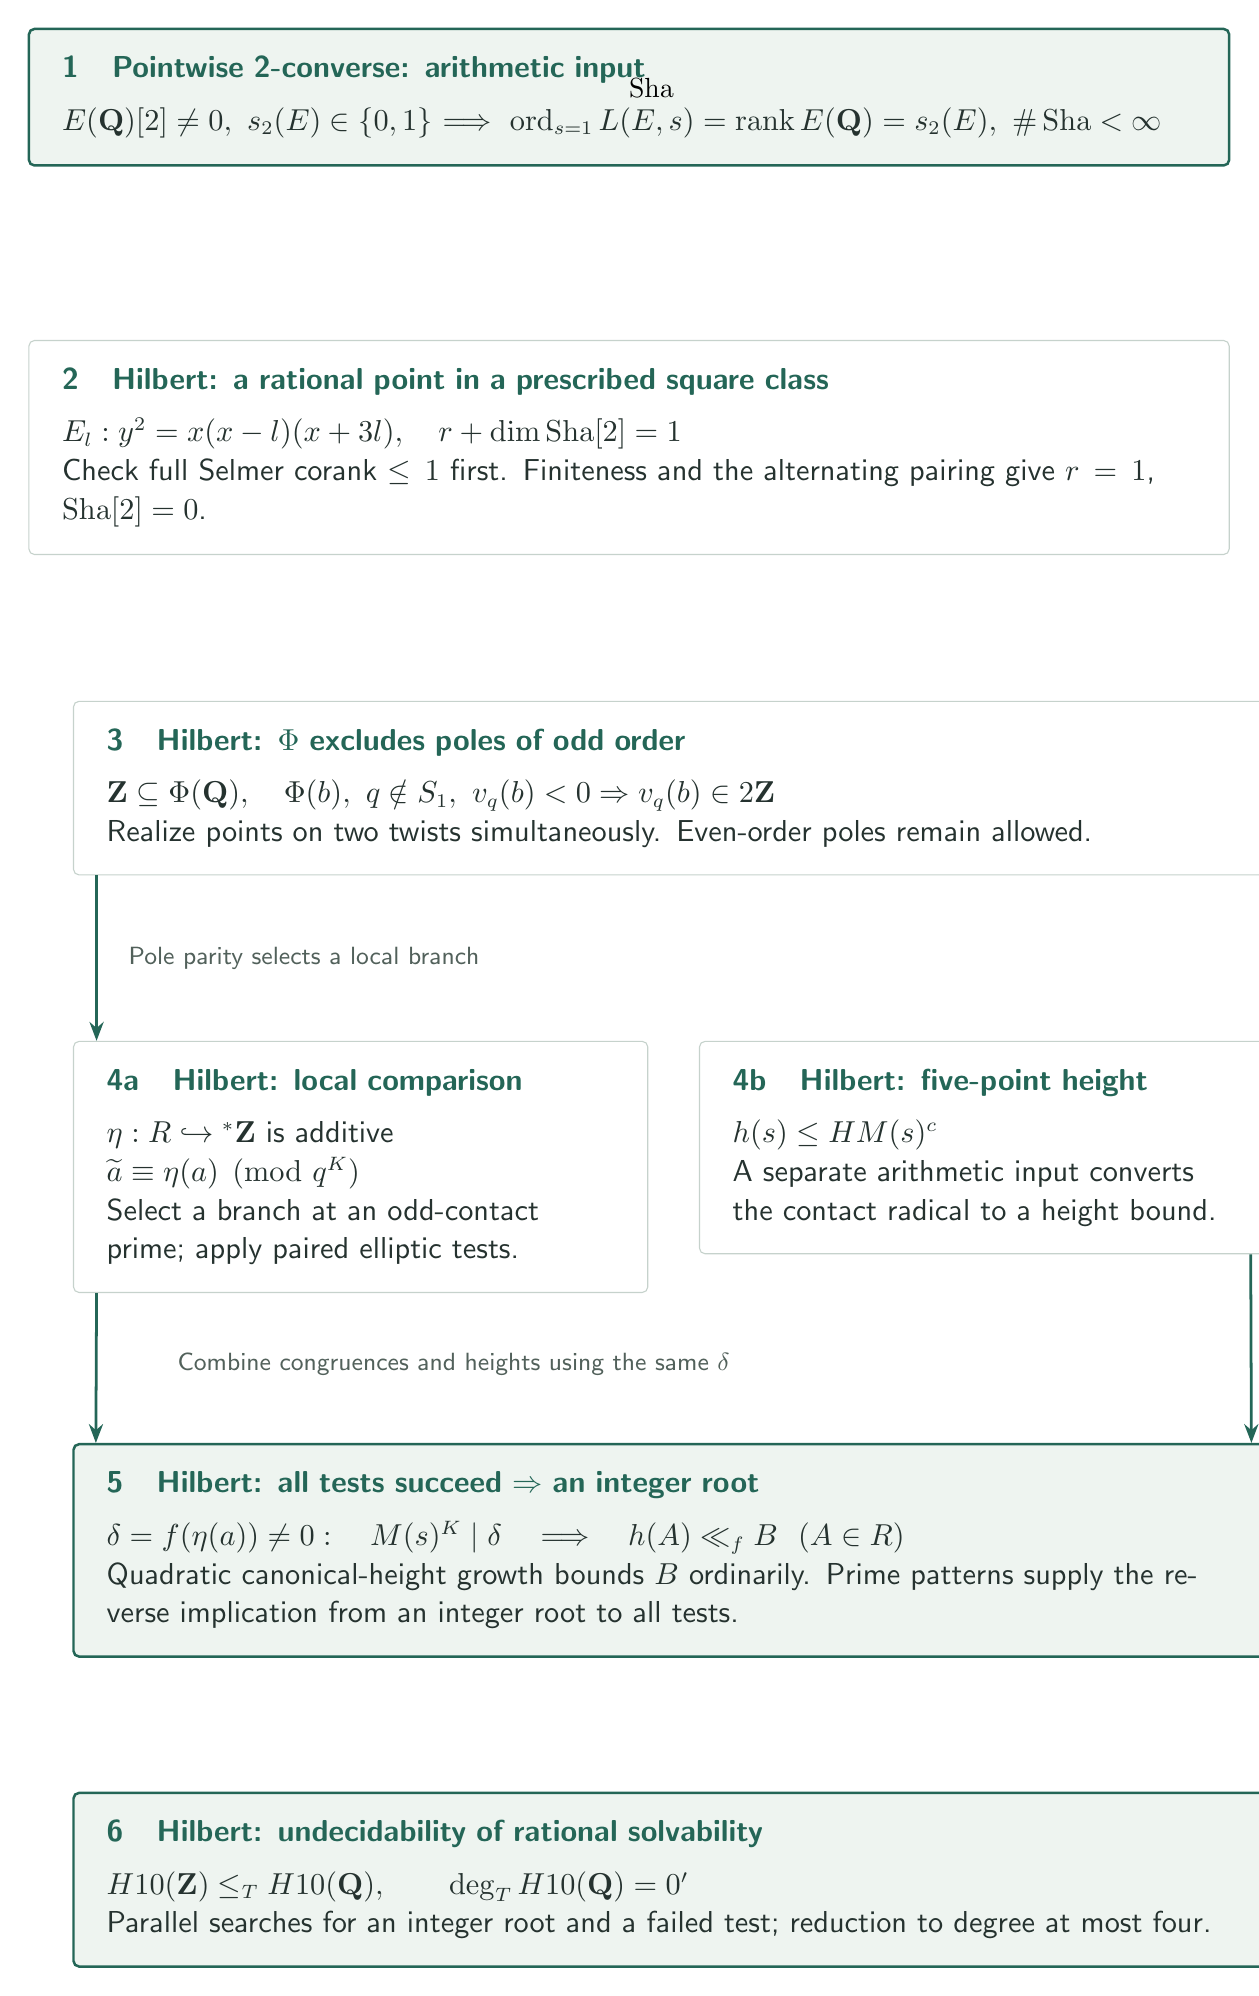
\begin{tikzpicture}
\node[result] (p) {\heading{1}{Pointwise 2-converse：算術入力}{Pointwise 2-converse: arithmetic input}
$E(\mathbf Q)[2]\ne0,\ s_2(E)\in\{0,1\}$
$\Longrightarrow\ \operatorname{ord}_{s=1}L(E,s)=\operatorname{rank}E(\mathbf Q)=s_2(E),\ \#\operatorname{Sha}<\infty$};
\node[card,below=2.2cm of p] (r) {\heading{2}{Hilbert：所定の平方類の有理点}{Hilbert: a rational point in a prescribed square class}
$E_l:y^2=x(x-l)(x+3l),\quad r+\dim\operatorname{Sha}[2]=1$\par
\Tx{full Selmer corank $\le1$ を先に確認。有限性と交代的 pairing から $r=1$, $\operatorname{Sha}[2]=0$。}{Check full Selmer corank $\le1$ first. Finiteness and the alternating pairing give $r=1$, $\operatorname{Sha}[2]=0$.}};
\flow{p}{r}{\Tx{直接入力：$\operatorname{Sha}$ 有限性を使い、Selmer類を有理点へ移す}{Direct input: use finite $\operatorname{Sha}$ to realize the Selmer class}\\[3pt]\Cite{pointwise-main}\\[3pt]\Cite{hilbert-transfer}};
\node[card,below=1.85cm of r] (phi) {\heading{3}{Hilbert：奇数位数の極を排除する $\Phi$}{Hilbert: $\Phi$ excludes poles of odd order}
$\mathbf Z\subseteq\Phi(\mathbf Q),\quad \Phi(b),\ q\notin S_1,\ v_q(b)<0\Rightarrow v_q(b)\in2\mathbf Z$\par
\Tx{二つのtwistで同時に有理点を実現する。偶数位数の極は許す。}{Realize points on two twists simultaneously. Even-order poles remain allowed.}};
\flow{r}{phi}{\Tx{同一パラメータで整数の証人を構成する}{One parameter supplies witnesses for every integer}\\[3pt]\Cite{hilbert-completion}\\[3pt]\Cite{hilbert-poles}};
\node[half,below=2.1cm of phi.south west,anchor=north west,xshift=0cm] (local) {\heading{4a}{Hilbert：局所比較}{Hilbert: local comparison}
$\eta:R\hookrightarrow{}^*\mathbf Z$ \Tx{は加法的}{is additive}\par
$\widetilde a\equiv\eta(a)\pmod{q^K}$\par
\Tx{奇接触素数で分岐を選び、対の楕円局所テストを適用。}{Select a branch at an odd-contact prime; apply paired elliptic tests.}};
\node[half,anchor=north east] (height) at ($(phi.south east)+(0,-2.1)$) {\heading{4b}{Hilbert：五点の高さ}{Hilbert: five-point height}
$h(s)\le H M(s)^c$\par
\Tx{接触素数の積を高さへ変える独立の算術入力。}{A separate arithmetic input converts the contact radical to a height bound.}\\[3pt]\Cite{hilbert-height}};
\draw[edge] ($(phi.south west)+(.3,0)$)--($(local.north west)+(.3,0)$);
\node[reason,anchor=west] at ($(phi.south west)+(.7,-1.05)$) {\Tx{極の偶奇から局所分岐へ}{Pole parity selects a local branch}\\[3pt]\Cite{hilbert-local}};
\node[result,below=2.15cm of $(local.south)!.5!(height.south)$] (tests) {\heading{5}{Hilbert：全テスト成功から整数根へ}{Hilbert: all tests succeed $\Rightarrow$ an integer root}
$\delta=f(\eta(a))\ne0:\quad M(s)^K\mid\delta\quad\Longrightarrow\quad h(A)\ll_f B\ \ (A\in R)$\par
\Tx{標準高さの二次増大が $B$ を通常の範囲に抑える。整数根から全テストへの向きには素数パターンを使う。}{Quadratic canonical-height growth bounds $B$ ordinarily. Prime patterns supply the reverse implication from an integer root to all tests.}};
\draw[edge] ($(local.south west)+(.3,0)$)--($(tests.north west)+(.3,0)$);
\draw[edge] ($(height.south east)+(-.3,0)$)--($(tests.north east)+(-.3,0)$);
\node[reason,anchor=center] at ($(tests.north)+(0,1)$) {\Tx{同一の $\delta$ へ合同と高さを合流させる}{Combine congruences and heights using the same $\delta$}\\[3pt]\Cite{hilbert-tests}};
\node[result,below=1.7cm of tests] (end) {\heading{6}{Hilbert：有理零点の決定不能性}{Hilbert: undecidability of rational solvability}
$H10(\mathbf Z)\le_T H10(\mathbf Q),\qquad \deg_T H10(\mathbf Q)=0'$\par
\Tx{整数根探索と失敗テスト探索を並走。次数4以下へも帰着。}{Parallel searches for an integer root and a failed test; reduction to degree at most four.}};
\flow{tests}{end}{\Tx{各テストは有限回の有理零点問い合わせで判定}{Each test uses finitely many rational-solvability queries}\\[3pt]\Cite{hilbert-degree}};

\end{tikzpicture}
\end{document}
